\section{Понятие качества программного обеспечения}

Существуют различные подходы к трактовке понятия качества программного обеспечения. Международный стандарт ISO 8402:94, например вводит качество программного обеспечения как "весь объем признаков и характеристик программ, который относится к их способности удовлетворять установленным или предполагаемым потребностям"  -- \cite{ISO840294}. Стандарт IEEE Std 610.12-1990 определяет качество ПО как "степень, в которой система, компонент или процесс удовлетворяют потребностям или ожиданиям заказчика или пользователя" -- \cite{1990ieee}

Однако исторически, первой записью о качестве продукта можно считать определение Уолтера Шухарта(англ. Walter Andrew Shewhart) в книге \cite{shewhart1931economic} качества как сущности, состоящей из двух аспектов. Один из них имеет дело рассмотрением качества как объективного факта, не зависящего от существования человека. Другой же, напротив, имеет дело с чувственными ощущениями реальности. Тем самым, Шухарт подводит нас к мысли, что у качества есть субъективная сторона.

Далее мысль Шухарта развил Джеральд Вайнберг(англ. Gerald Marvin Weinberg) в своей работе 1992 года \cite{weinberg1993quality}, говоря о качестве, как о "значимом для какого-либо человека". Отсюда полезно задаться вопросом, какие люди будут оценивать качество отдельно взятого программного продукта и что будет ценным для них?

Отголосок этой мысли есть и в международном стандарте ISO/IEC 9126 -- \cite{ISOIEC9126}, который вводит так называемую модель качества, которая описывает различные подходы к нему в течение всего жизненного цикла ПО.

\begin{figure}[H]
  \centering
  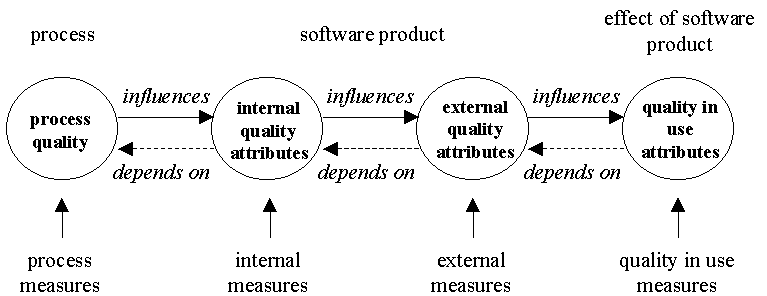
\includegraphics[width=\textwidth]{img/quality_framework.png}
  \caption{Модель качества, согласно ISO/IEC FDIS 9126-1}
\end{figure}

Уже при первом взгляде на эту модель становится понятно, что на различных этапах жизненного цикла ПО используются различные, понятия качества. Так, в ходе непосредственно разработки мы говорим о качестве \textit{процесса} разработки, которое напрямую влияет на внутреннее качество программного продукта.\footnote{Кроме того, я буду использовать термин "программный продукт", считая его синонимом для программы или программного обеспечения. Формально, это конечно же, неверно, но в нашем контексте это не играет большой роли.} Внутреннее качество продукта, в свою очередь, влияет на внешнее качество продукта, которое, затем, определяет качество продукта с точки зрения пользователя.

Может возникнуть вопрос, чем отличаются внутреннее качество продукта, от внешнего? Можно считать, что внутреннее качество программного обеспечения связано с некоторыми внутренними метриками(метриками, которые можно получить не запуская программу). Внешнее качество, соответственно, связано с внешними метриками(например, как ведет себя запущенная в некотором внешнем окружении программа).

В рамках внутреннего и внешнего качества стандарт предлагает следующие характеристики, приведенные на рисунке ниже:

\begin{figure}[H]
  \centering
  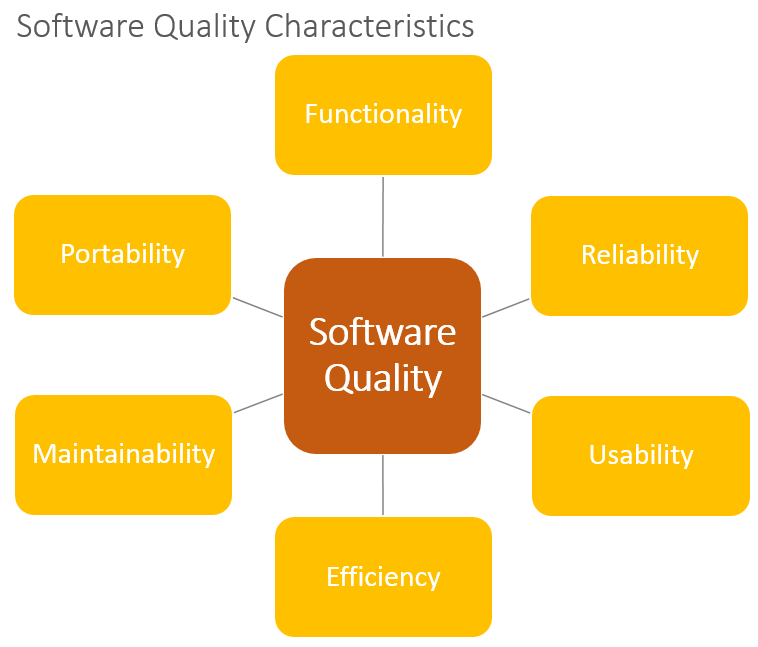
\includegraphics[width=\textwidth]{img/quality_model.png}
  \caption{Характеристики качества ПО, согласно ISO/IEC FDIS 9126-1}
\end{figure}

\begin{enumerate}
  \item Функциональность(\textit{Functionality}) определяется способностью ПО решать возложенные на него задачи, соответствующие потребностям пользователя при заданных условиях использования. То есть эта характеристика говорит о том, что программа работает исправно точно и безопасно.
  \item Надежность(\textit{Reliabilty}) определяется способностью программы штатно завершаться, восстанавливаться в случае сбоев в работе. Другими словами -- это способность программы выполнять требуемые задачи в обозначенных условиях, в течение обозначенных сроков.
  \item Удобство использования(\textit{Usability}) означает легкость в понимании и изучении ПО для пользователя. Эта характеристика больше относится к качеству ПО с точки зрения пользователя.
  \item Эффективность(\textit{Efficiency}) определяется способностью программы обеспечивать требуемый уровень производительности в условиях обозначенного времени или используемых ресурсов.
  \item Удобство сопровождения(\textit{Maintainability}) -- это легкость, с которой программу можно анализировать, тестировать изменять с целью исправления каких-либо дефектов или для адаптации к новому окружению.
  \item Переносимость(\textit{Portability}) -- это способность программного обеспечения запускаться и работать вне зависимости от программного или аппаратного окружения.
\end{enumerate}

Нас будет интересовать в большей степени внутреннее качество ПО и способы его обеспечения, однако мы чуть-чуть коснемся и внешнего качества. Качество процесса разработки, равно как и качество ПО с точки зрения пользователя мы постараемся оставить за кадром.
